\documentclass[titlepage]{article}
\usepackage[margin=3cm]{geometry}
\usepackage{datetime}
\usepackage{fontspec}
\usepackage{graphicx}
\usepackage{hyperref}
\usepackage{kotex}
\usepackage[lighttt]{lmodern}
\usepackage{listings}
\usepackage{tikz}
\usepackage{sectsty}
\usepackage[edges]{forest}
\usepackage{float}
\usepackage{flowchart}

\usepackage[headsepline]{scrlayer-scrpage}
\newcommand{\doctitle}{CSED101: Assignment 2}
\clearpairofpagestyles
\ohead{\thepage}
\ihead{\doctitle}

\usetikzlibrary{arrows}
\usetikzlibrary{fit}

\setmainhangulfont{Noto Serif CJK KR}[
  UprightFont=* Light, BoldFont=* Bold,
  Script=Hangul, Language=Korean, AutoFakeSlant,
]
\setsanshangulfont{Noto Sans CJK KR}[
  UprightFont=* DemiLight, BoldFont=* Medium,
  Script=Hangul, Language=Korean
]
\setmathhangulfont{Noto Sans CJK KR}[
  SizeFeatures={
    {Size=-6,  Font=* Medium},
    {Size=6-9, Font=*},
    {Size=9-,  Font=* DemiLight},
  },
  Script=Hangul, Language=Korean
]
\lstset{
  numbers=none, frame=single, showspaces=false,
  showstringspaces=false, showtabs=false, breaklines=true, showlines=true,
  breakatwhitespace=true, basicstyle=\ttfamily, keywordstyle=\bfseries, basewidth=0.5em
}
\allsectionsfont{\sffamily}

\title{\doctitle}
\author{무은재학부 손량 (20220323)}
\date{Last compiled on: \today, \currenttime}

\begin{document}

\makeatletter
\begin{titlepage}
  \begin{center}
    \vspace*{3cm}
    \Huge
    \textsf{\@title}

    \vspace{1.5cm}
    \LARGE
    \@author

    POVIS ID: \texttt{ryangsohn}

    \vspace{0.5cm}
    담당 교수: 윤은영 교수님

    \vfill
    \large
    \textit{``나는 이 프로그래밍 과제를 다른 사람의 부적절한 도움 없이 완수하였습니다.''}
  \end{center}
\end{titlepage}

\section{문제의 개요}

본 프로그램은 ppm 형식의 이미지를 받아 색조를 변경하고, 히스토그램과 이미지를 출력하거나 저장하는 기능을 C언어로 구현한 것이다. 이 프로그램의 structure chart는 다음과 같다.\footnote{지면을 아끼기 위해 프로그램의 기능상 중요한 함수들 위주로 structure chart에 넣었다.}

\begin{figure}[H]
  \centering
  \begin{forest}
    for tree={
      draw,
      align=center,
      grow=east
    },
    forked edges,
    [ASSN2: 이미지 색조 변경
      [\texttt{load\_image}
        [\texttt{rgb\_to\_hsv}
        ]
      ]
      [\texttt{save\_image}
      ]
      [\texttt{print\_image}
        [\texttt{set\_output\_color\_rgb}
        ]
        [\texttt{reset\_output\_color}
        ]
      ]
      [\texttt{print\_histogram}
        [\texttt{quantize\_hue}
        ]
        [\texttt{hsv\_to\_rgb}
        ]
      ]
      [\texttt{change\_color}
      ]
    ]
  \end{forest}
\end{figure}

\section{프로그램 구조 및 설명}

본 프로그램에서 사용한 알고리즘을 pseudocode로 나타내면 다음과 같다.

\begin{lstlisting}
create variable for filename, image_rgb, image_hsv, width, height
get filename from standard input
load ppm file from filename
if load failed:
  print error message
  quit
create variable finish and set to false
while not finish:
  create variable input
  get user input to input
  if input is invalid:
    go back to get user input
  if input == 1:
    print histogram of image
  else if input == 2:
    print histogram of image
    create variable source, target
    get source and target from standard input
    if source or target is invalid:
      go back to get source and target
    change color of image according to source and target
    convert HSV image to RGB image
  else if input == 3:
    print image to the terminal
  else if input == 4:
    save the image to "output.ppm"
  else if input == 5:
    set finish to true
\end{lstlisting}

Flowchart로 나타내면 다음과 같다.

\begin{figure}[H]
  \centering
  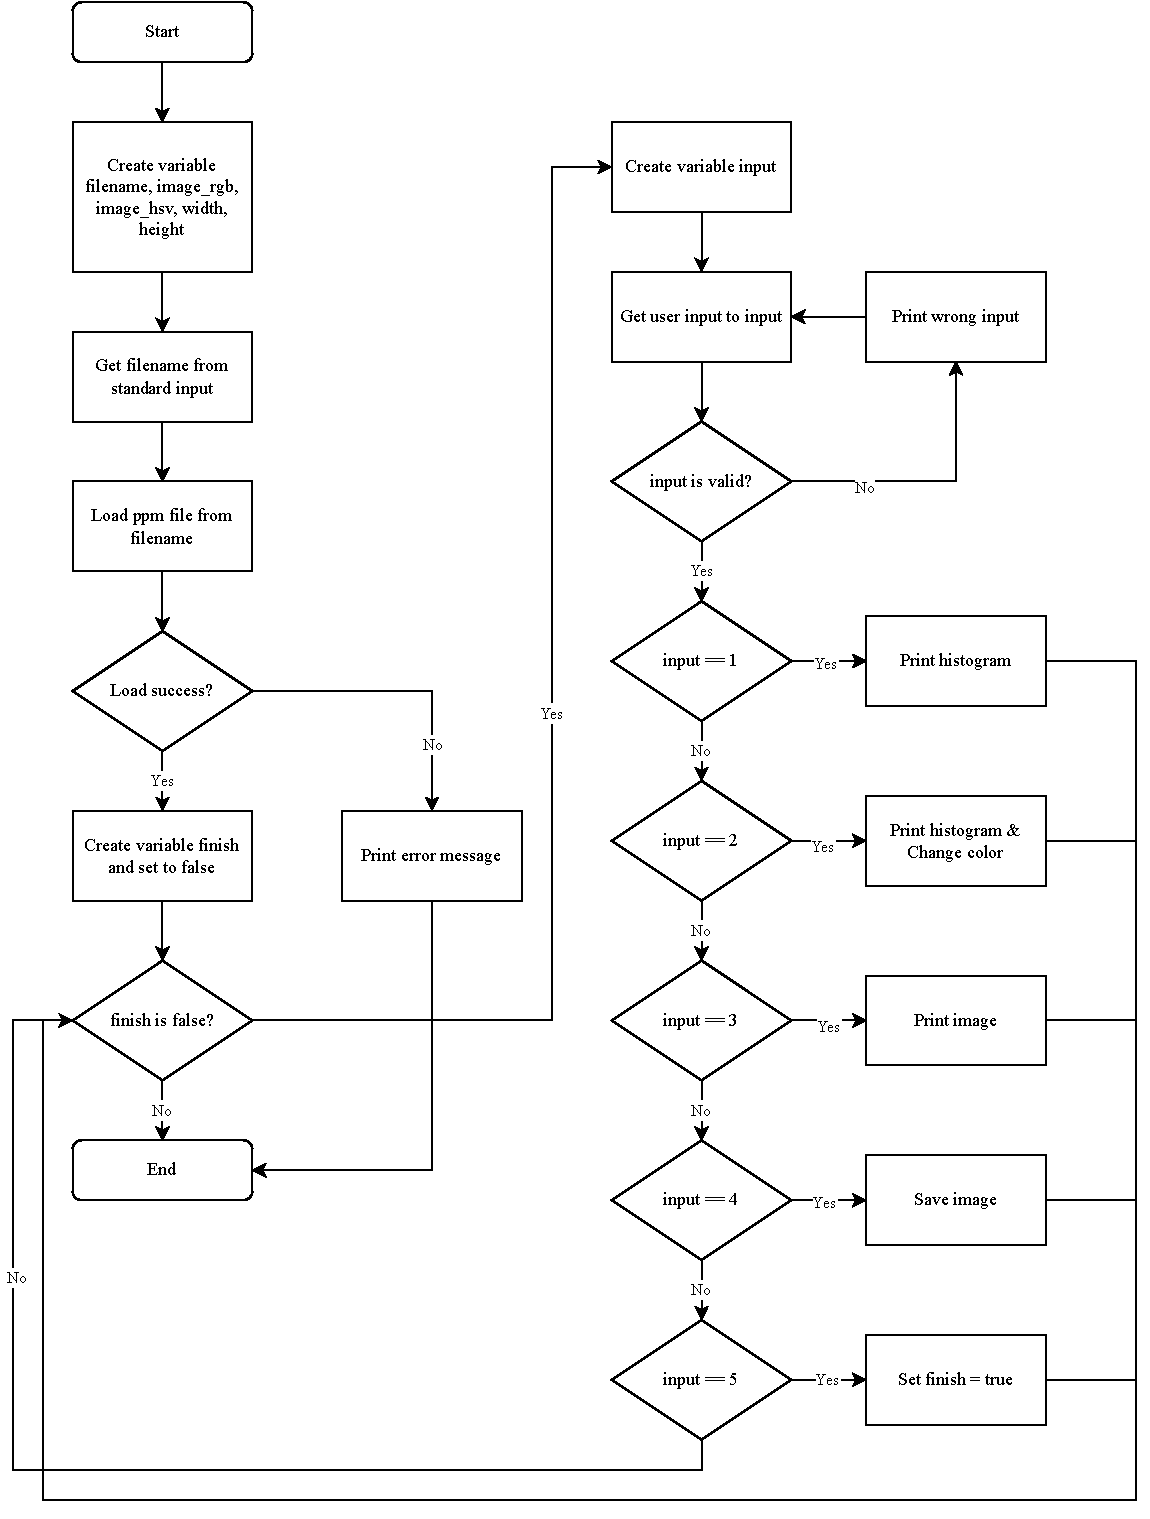
\includegraphics[width=0.9\linewidth]{flowchart.drawio.pdf}
\end{figure}

\section{프로그램 실행 방법과 예제}

첨부한 \texttt{assn2.c} 파일은 Linux, macOS 등의 UNIX 계열 OS에서 실행하는 것을 전제로 작성되었다.\footnote{Windows의 경우 WSL이나 Cygwin 등의 환경에서 실행할 수 있을 것이다.} \texttt{gcc} 컴파일러가 설치된 환경에서는 다음 명령어를 통해 코드를 컴파일할 수 있다.

\begin{lstlisting}
$ gcc -o assn2 assn2.c
\end{lstlisting}

이때 프로그램을 실행한 모습은 다음과 같다.

\begin{figure}[H]
  \centering
  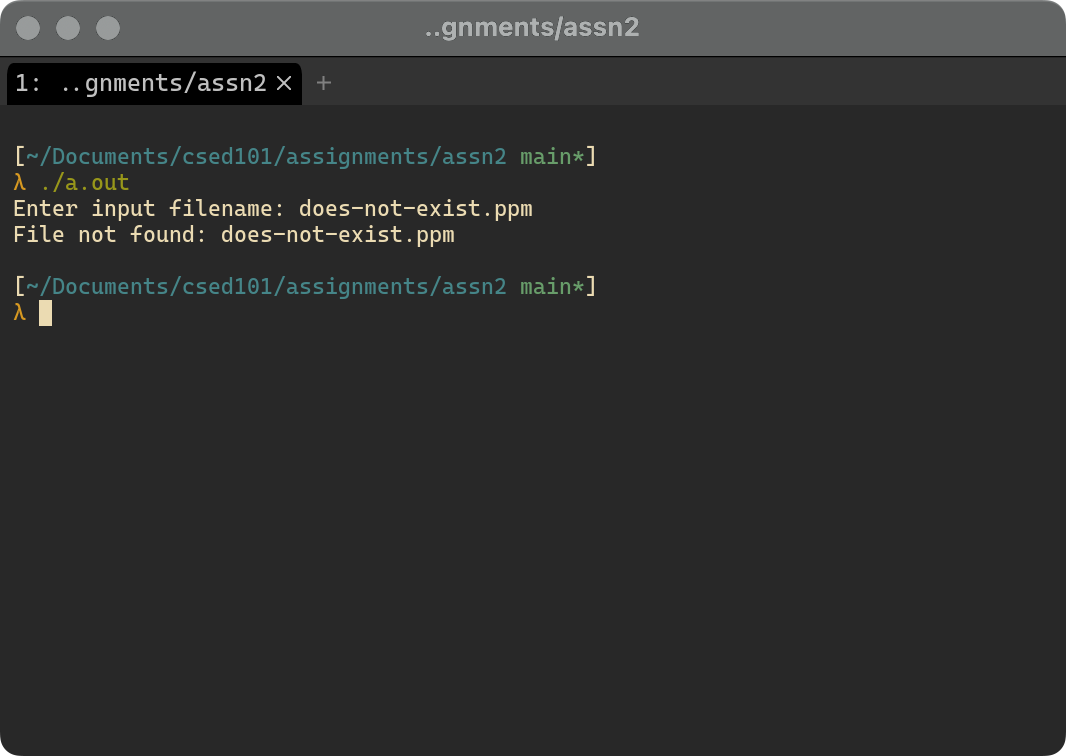
\includegraphics[width=0.7\linewidth]{file_check.png}
  \caption{존재하지 않는 파일을 열려고 시도했을 때.}
\end{figure}

\begin{figure}[H]
  \centering
  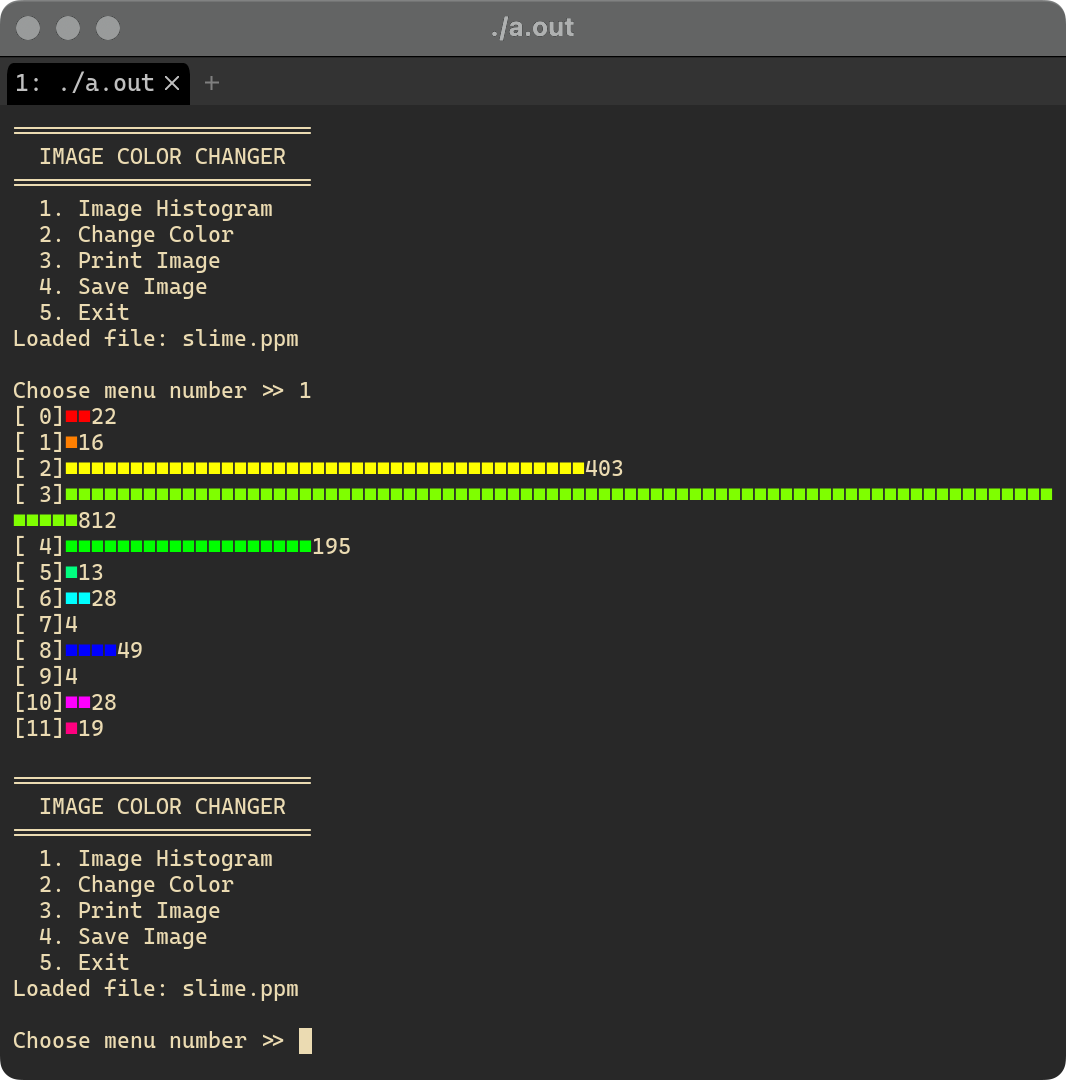
\includegraphics[width=0.7\linewidth]{histogram.png}
  \caption{샘플 이미지 \texttt{slime.ppm}의 히스토그램.}
\end{figure}

\begin{figure}[H]
  \centering
  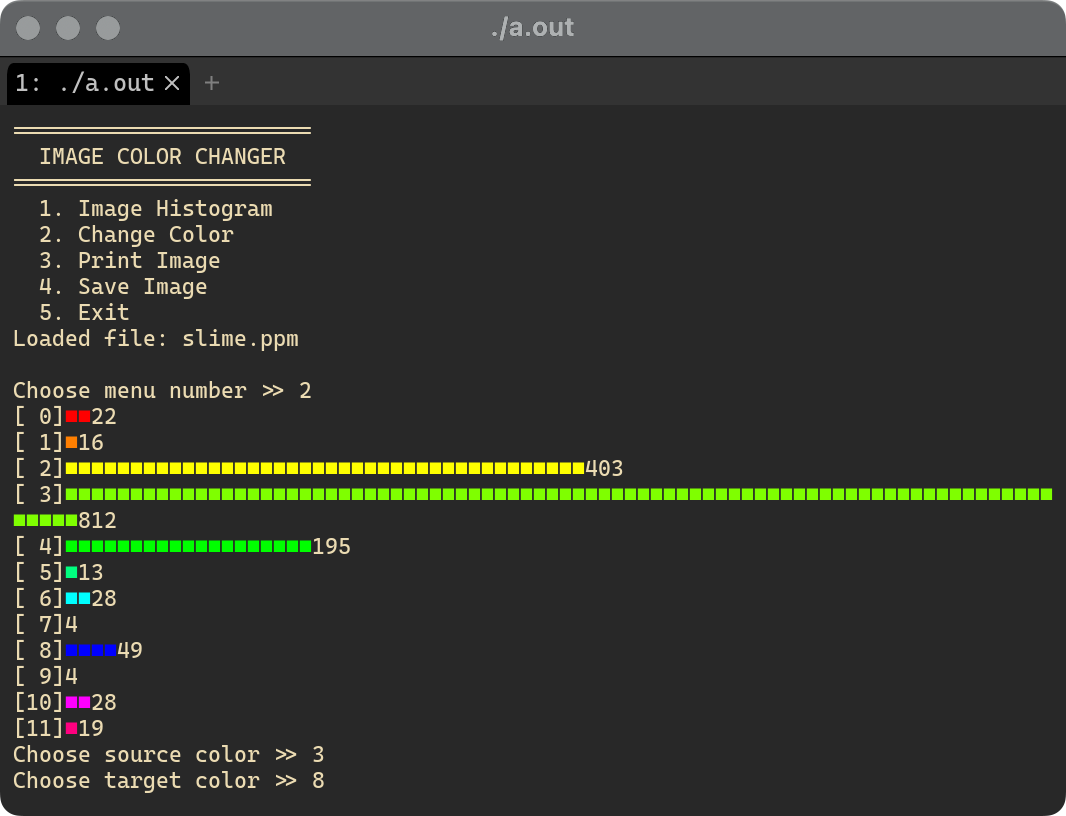
\includegraphics[width=0.7\linewidth]{change_color.png}
  \caption{이미지 색 변경을 하는 모습.}
\end{figure}

\begin{figure}[H]
  \centering
  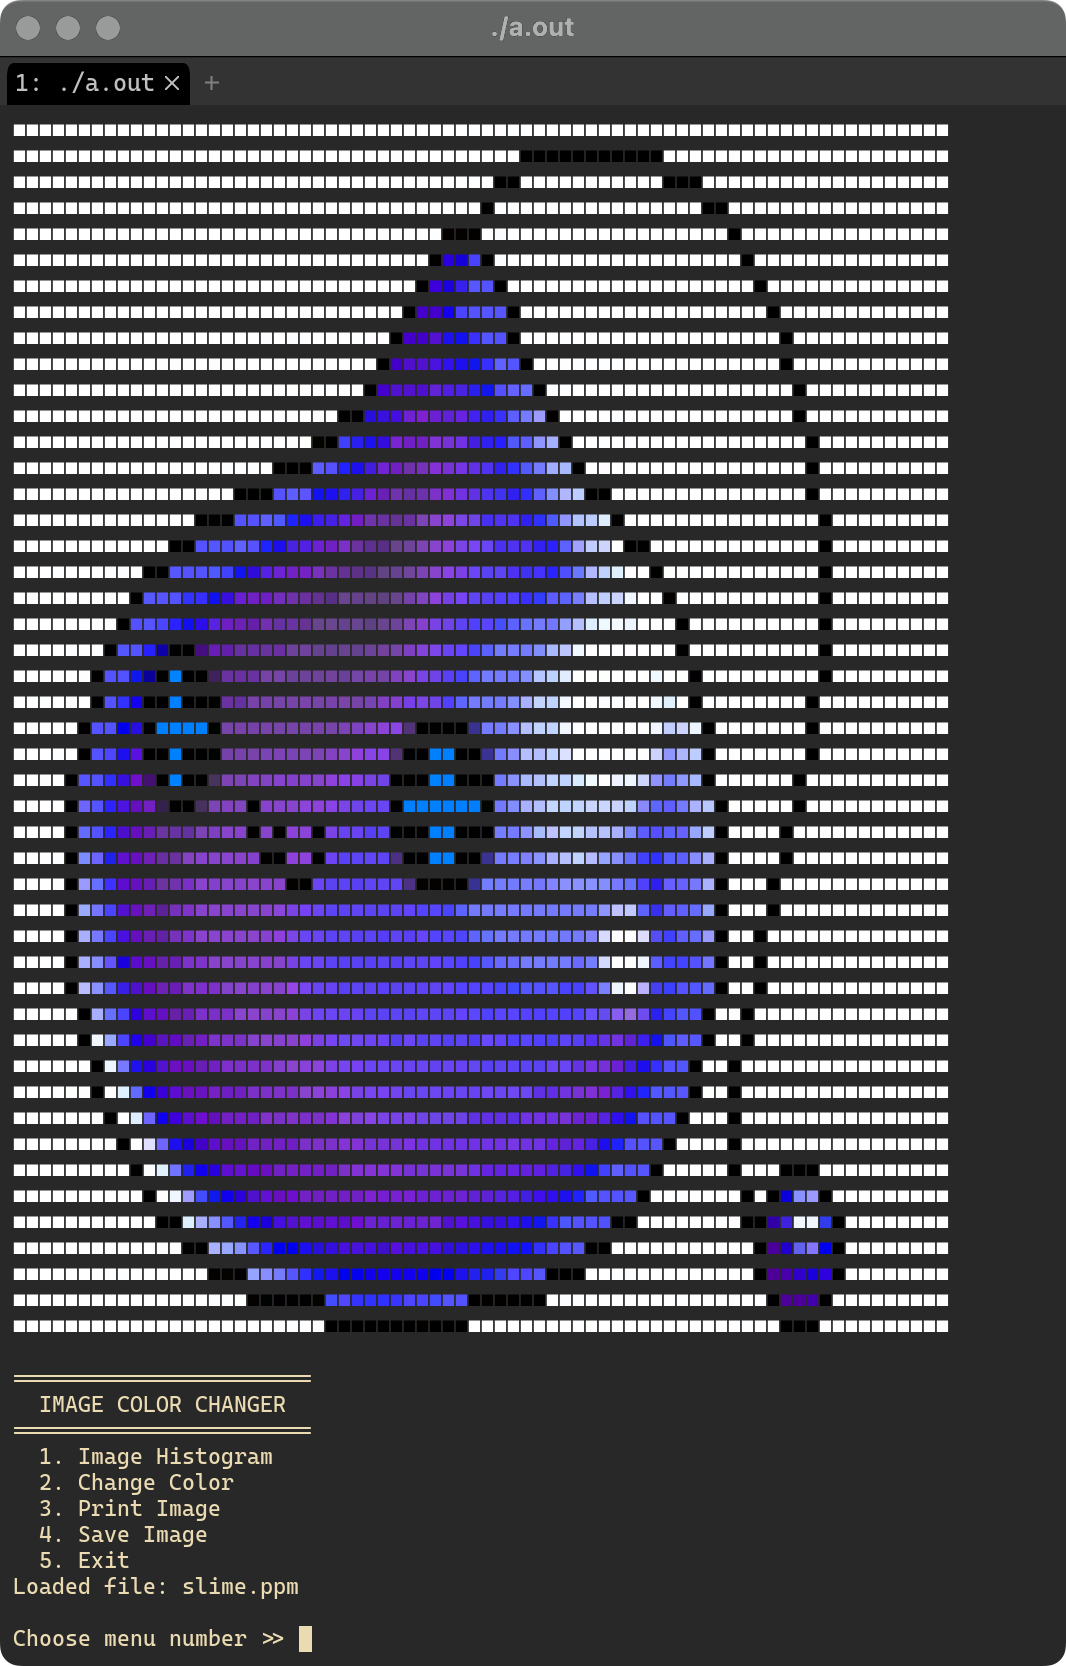
\includegraphics[width=0.7\linewidth]{change_color_result.png}
  \caption{색을 변경한 이미지를 출력한 것.}
\end{figure}

\begin{figure}[H]
  \centering
  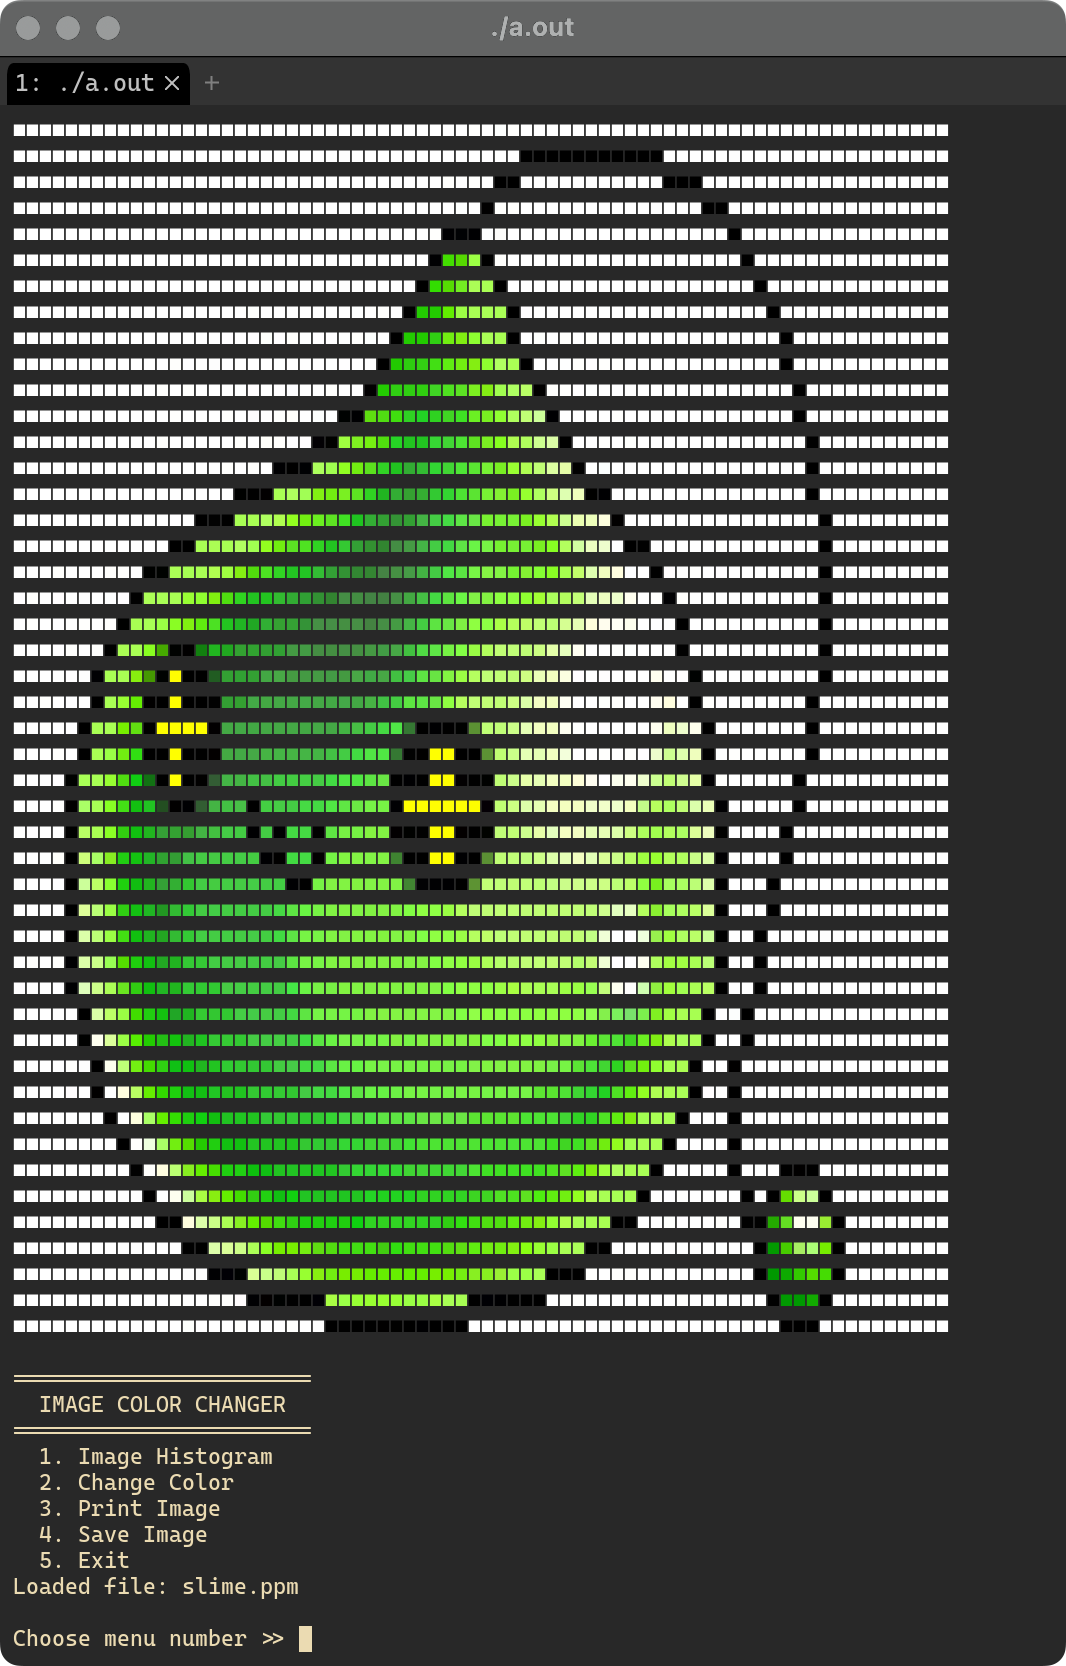
\includegraphics[width=0.7\linewidth]{print_image.png}
  \caption{샘플 이미지 \texttt{slime.ppm}을 출력한 것.}
\end{figure}

\begin{figure}[H]
  \centering
  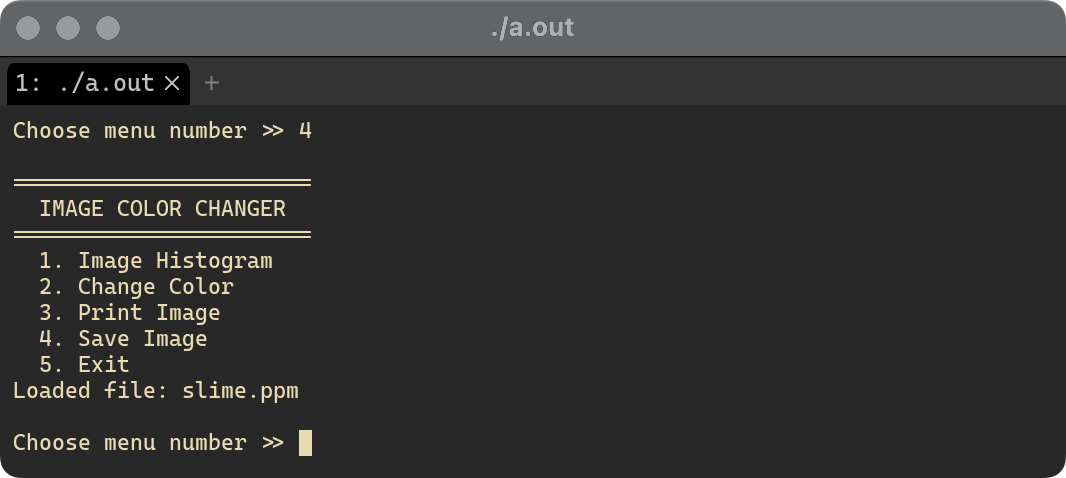
\includegraphics[width=0.7\linewidth]{save_image.png}
  \caption{이미지를 저장하는 모습.}
\end{figure}

\section{토론}

\subsection{히스토그램 계산}

히스토그램의 범위당 도수를 \texttt{pixel\_count} 배열에 저장하였고, 이 배열의 인덱스를 계산히기 위하여 \texttt{quantize\_hue} 함수를 구현하였다. 이 함수는 \(H\)값이 주어졌을 때 30으로 나눈 다음 버림하여 0 이상 11 이하의 정수를 반환한다.

\subsection{HSV-RGB 색 변환}

HSV 색공간에서 RGB 색공간으로 변환할 때, \(H\)값의 범위에 따라 \(R', G', B'\)값을 정하는 부분이 있다. 이를 단순히 \texttt{if}문으로 구현할 수도 있지만, 식에서의 대칭성에 주목할 수 있다. \texttt{quantize\_hue} 함수의 반환값이 \(\hat{H}\) 일때, \(R', G', B'\)값은 다음과 같이 정해진다.

\begin{figure}[H]
  \centering
  \begin{tabular}{|c|cccccccccccc|}
    \hline
    \(\hat{H}\) & 10    & 11    & 0     & 1     & 2     & 3     & 4     & 5     & 6     & 7     & 8     & 9     \\
    \hline
    \(R'\)      & \(C\) & \(C\) & \(C\) & \(C\) & \(X\) & \(X\) & 0     & 0     & 0     & 0     & \(X\) & \(X\) \\
    \(G'\)      & 0     & 0     & \(X\) & \(X\) & \(C\) & \(C\) & \(C\) & \(C\) & \(X\) & \(X\) & 0     & 0     \\
    \(B'\)      & \(X\) & \(X\) & 0     & 0     & 0     & 0     & \(X\) & \(X\) & \(C\) & \(C\) & \(C\) & \(C\) \\
    \hline
  \end{tabular}
\end{figure}

\(R', G', B'\) 값을 길이 3짜리 배열에 넣는다고 하자. 이때 \(C\)가 저장되는 인덱스는 10부터 \(\hat{H}\)가 4 증가할 때마다 1씩 증가하고, \(X\)가 저장되는 인덱스는 2 증가할 때마다 2-1-0-2-1-0 패턴으로 바뀐다. 나머지, 나누기 연산자를 잘 이용하면 조건 분기 없이 이 규칙에 따라 값을 정할 수 있다. 대부분의 프로세서는 조건 분기가 없는 코드를 잘 실행하기 때문에, 이로 인한 성능 향상까지도 기대할 수 있을 것이다.

\subsection{실수 오차 처리}

과제 문서에도 나와 있지만, 부동소수점 실수의 오차를 감안하여 비교할 수 있도록 \texttt{compare\_f} 등 오차를 고려하는 비교 함수를 코딩하여 곳곳에서 사용하였다.

\section{결론과 개선 방향}

C언어를 활용하여 이미지의 색조를 변환하는 프로그램을 작성하였다. 프로그램은 잘 동작하지만, 몇 가지 개선할 만한 점을 여기 적어 보았다.

\subsection{큰 이미지 지원}

현재 프로그램이 지원하는 최대 이미지 크기는 가로세로 75픽셀이다. 하지만 이러한 이미지 크기는 1080p, 4K 모니터들이 대중화된 현대의 기준에서는 매우 작다. 이 프로그램도 이에 맞추어 더 큰 크기의 이미지를 지원할 필요가 있을 것이다. 하지만, 이는 단순히 \texttt{main}함수에서 선언하는 \texttt{image\_rgb}, \texttt{image\_hsv} 등의 배열 크기를 키워서 해결되지는 않는다. 프로그램이 사용하는 스택 크기를 초과할 가능성이 있을 뿐만 아니라, 프로그램이 시작할 때 그렇게 큰 메모리를 스택에 할당받는 것은 비효율적이고, 공간의 낭비로 이어질 가능성이 있기 때문이다. 이를 해결하기 위해서는 동적 메모리 할당을 사용하거나, 이미지가 메모리에 들어가지 않는 경우에는 디스크 기반 저장소를 사용하는 것도 검토해야 할 것이다.

\subsection{성능 최적화}

최근 출시되는 CPU는 AVX, NEON, SVE 등 vector instruction set을 지원하여 배열에서 여러 개의 원소를 한꺼번에 처리할 수 있다. 이 프로그램에서도 히스토그램 계산, 색조 변경 등 이미지의 모든 픽셀에 대해 반복하는 부분들이 많이 있는데, 이러한 작업은 trivially vectorizable task 이므로 큰 어려움 없이 좋은 성능을 내는 코드를 작성할 수 있을 것이다.

\end{document}
